\section{Workflows}
\label{s:workflows}

We designed and implemented three realistic online workflows based on
scientific codes having large user bases: the LAMMPS Newtonian particle
simulator~\cite{plimpton:1997:lammps}, GTCP, a particle-in-cell Tokamak
simulator~\cite{lin:gtc}, and GROMACS,
a biomolecular dynamics code~\cite{hess2008gromacs}.
While all these workflows eventually turn part of the
simulation data into histograms of certain quantities of interest,
there is significant variation in 
how they
arrive at their final result.
Creating similar types of results, and this using some
of the same components but in significantly
different ways, has allowed us to gain important insight into how best to
design components that can be used to build a wide variety of workflows.
We first describe the workflows from a general point of view
and then the components in greater detail, illustrated
in~\autoref{fig:lammps-workflow} ~\autoref{fig:gtcp-workflow}
and~\autoref{fig:gromacs-workflow}.

\subsection{LAMMPS Workflow}

We configure LAMMPS to simulate a disruption (a ``crack'') in a thin layer of
particles and output 5 numerical properties describing each particle in the
simulation at regular timestep intervals. This corresponds to two-dimensional
data (particles as one dimension and properties of interest as another) and
among these properties are the three-dimensional components of the particles'
velocities. The workflow outputs one histogram per timestep
showing the distribution of the magnitudes of the particles' velocities
for all particles involved in simulation at that point in
time.

\subsection{GTCP Workflow}

\begin{figure}
  \centering
  \vspace{-0.10in}
  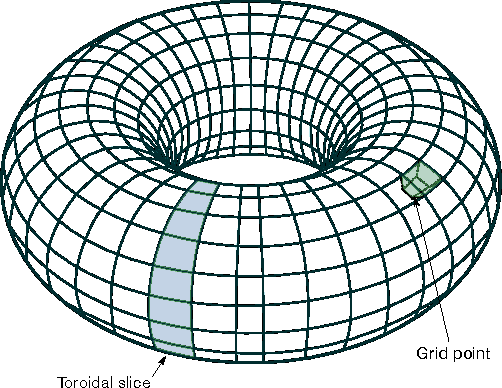
\includegraphics[width=0.7\columnwidth]{fig/Simple_Torus_mod}
  \vspace{-0.09in}
  \caption{Representation of GTCP Toroid, modification of \cite{WikimediaCommons:torus}}
  \label{fig:toroid}
  \vspace{-0.20in}
\end{figure}

GTCP, a code that simulates a toroidally confined plasma, splits the solid into
toroidal slices, each made up of a number of grid points. For each of these
grid points, it outputs 7 properties of the plasma such as pressure and energy
flux. This division of the toroid is illustrated in~\autoref{fig:toroid}.
The output of the simulation is therefore a three-dimensional array in which
the dimensions span: (a) toroidal ranks (toroidal slice number), (b) grid point
numbers, and (c) various properties that describe each grid point.
In this workflow, the per-timestep histogram
generated shows the distribution of per-gridpoint perpendicular pressures across
the entire simulation.

\subsection{GROMACS Workflow}

Among other quantities, GROMACS outputs
the three-dimensional positions
of the atoms involved in the simulation
at regular intervals.
From these, we obtain a histogram of the distances
of the atoms from the origin for each timestep, showing
an evolution of the spread of the particles through
the simulation in a human-readable way.

\subsection{Discussion}

All three workflows are built using only the simulation code,
modified to allow for ADIOS output, as well as SuperGlue
components, unchanged when the same component is used
in different workflows.
As we will explain in more detail later,
the components' ability to fit
into different workflows
is achieved using command-line
parameters specified in the batch job
submission script used for launching
the whole workflow on the target cluster.

All three workflows create histograms as their final
result, as histograms are a common final,
human-readable result of many types of workflow.
However, the components presented in this paper
are meant only to illustrate the building blocks
of a library of such tools, of which histogram is
only an example.

Also, the driving simulations generate very
different data, so selecting the
relevant data from the simulations and
formatting it in a such a way that the
final Histogram component can operate on
it is done differently in each
workflow.

Much of the challenge is the
data selection and mathematical
manipulation to obtain the quantities of
interest in a way that (a) presents an
intuitive interface to the scientist
constructing the workflow and (b) is
useful in different types of workflows
in which data have different sizes and
dimensions.  This difficulty arises
because (a) the data at each stage of the
workflow is distributed over the collection
of processes, with varying levels
of parallelism at each stage, and
(b) the extraction and
re-arrangement of multi-dimensional,
distributed data, in a way that is
configurable by the user at runtime is challenging. 

Addressing these challenges has offered us some insight
in the design of such generic tools.

\if 0
\subsection{Discussion}

In both cases, a particular subset of interest is extracted from the
output data set, a calculation is performed, and a histogram is
generated. This is illustrated in~\autoref{fig:generic-workflow}. In many
cases, the histogram component may be some standard, reusable operator.
The challenge is the data selection and mathematical
manipulation to obtain the quantities of interest in a way that (a) presents an
intuitive interface to the scientist constructing the workflow and (b) is
useful in different types of workflows in which data have different sizes and
dimensions.  This difficulty arises because (a) the data at each stage of the
workflow is distributed over the collection of processes involved in each
component even if it forms a coherent whole and (b) the extraction and
re-arrangement of multi-dimensional, distributed data, in a way that is
configurable by the user at runtime is challenging.  Both workflows are
similar, insofar as both codes generate a large output while we are only
interested in a per-timestep histogram of a particular simulation quantity.
However, because the simulations generate very different data, selecting the
relevant data from the simulations and formatting it in a such a way that the
final Histogram component can operate on it is done very differently in each
workflow.

\begin{figure}[htbp]
  \vspace{-0.1in}
  \centering
  \includegraphics[width=0.7\columnwidth]{fig/gwflow}
  \vspace{-0.09in}
  \caption{Generic Workflow Illustration}
  \label{fig:generic-workflow}
  \vspace{-0.10in}
\end{figure}

In typical scientific workflows today, custom glue code is written for
selecting relevant data and writing it so the ``formatter'' illustrated in~\autoref{fig:generic-workflow} can work.  Then, potentially additional
custom glue code will fix the histogram calculation into something that can be
rendered or saved as desired.  In this work, we demonstrate general, reusable
components capable of handling all three intermediate operations.

The workflows presented here use no custom glue code. Instead, the glue is
designed as generic components that accept command-line configuration options
at launch time. At most, the user specifies a few parameters and organizes
the components into a proper pipeline. Both of these operations are easy enough
that a non-expert
%application scientist
can create workflows through GUIs or other guided assembly techniques.

That we are able to use some of the same glue code to connect the start to the
end of each workflow shows that generic glue code that can manipulate large
datasets in real time is possible and useful for assembling very different
workflows.  In addition, we later show that generic components, both glue and
analytical, have the advantage of possessing known performance characteristics,
which greatly facilitates the configuration of workflows that use them.
\fi

